\documentclass[10pt,halfline,a4paper]{ouparticle}
\usepackage{url}
  \let\oldurl\url

\usepackage{hyperref}
 \let\linkurl\url
  \let\url\oldurl
\usepackage[table]{xcolor}
\usepackage{color}
\usepackage{natbib}

\usepackage{graphicx}
\usepackage{wrapfig}
\usepackage{lscape}
\usepackage{rotating}


\usepackage{fancyhdr}

\pagestyle{fancy}
\fancyhf{}
\fancyhead[LE,RO]{}
\fancyhead[RE,LO]{}
\fancyfoot[CE,CO]{\leftmark}
%\fancyfoot[LE,RO]{\thepage}

\renewcommand{\headrulewidth}{2pt}
\renewcommand{\footrulewidth}{1pt}




\begin{document}

\title{A Risk Methodology and Tool for Managing Risks incurred in Large Scale Construction Projects}

\author{%
\name{Nam Lethanh \footnote{PhD, Director, Arcadis Philippines Inc. (le.nam@arcadis.com)} \footnote{Senior Lecturer \& Data Scientist, Head of Urban Resilience and Risk Management, Institute of Smart City and Management, University of Economics Ho Chi Minh, Vietnam. (namlt@ueh.edu.vn}} 
\address{\href{https://namkyodai.github.io/}{https://namkyodai.github.io/}}
%\address{Principal, infraPLUS Consulting Ltd., Vietnam}
%\email{namlt@protonmail.ch and nam.lethanh@ghd.com}
}

\abstract{In development phases of large scale construction projects, various types of hazards and uncertainties could occur that negatively impact the overall performance of the projects (e.g. cost, time, quality, safety, community). Combinations of hazards and impacts are risks that need to be identified, ranked, controlled for elimination or mitigation. To execute this task, it is important at the outset to develop an appropriate risk management approach that shall address risks incurred by involved stakeholders (e.g. the Owners, Contractors, and the Public). It should also considers its feasibility regarding implementation in local context and culture as stakeholders have different backgrounds in doing business and culture as well as understanding on the methodological approach itself.
	
The proposed risk management approach in this work has been developed, tested, and implemented in a large scale Design and Build project. The approach includes a risk register component and then rank risks into level of intensity and consequence. The intensity and consequence are in five discrete scale resulting in having 25 levels of risks. The higher the intensity and consequence are, the higher risk becomes. Risks are also grouped per matrices of phases and responsibilities that are intuitive and convenient for project team members and managers to comprehend, therefore, helping the team and managers in making optimal decisions regarding how to eliminate and mitigate risks.}

\date{\today}

\keywords{risk control; risk management; water treatment plant, design and build}

\maketitle


\section{Introduction}
\label{sec1}
In large scale Design and Build (D\&B) projects, there exists a vast number of uncertainties and potential hazards that if they are occurred, may lead to significant consequences and losses. As uncertainties of events and hazards occur in a certain range of probability,  risks are then the multiplication of the probability and measurable consequences the hazard events might trigger. In order to minimize and mitigate risks incurred in a large scale construction project, which is the mandate of all project stakeholders (owners, contractors, consultants, and other private and public entities), a feasible and practical risk management methodology must be tailored to suit the expectation of stakeholders regarding the requirements for risk management. Moreover, a risk tool must be developed based explicitly on the methodology to be appropriately used in practical situations. 




\section{Background}
\label{sec2}
Risk management is one of the important pillars of project management \citep{PMI2003}. This is practically true for a large scale construction project, in which stakeholders of the project have to confront with daily hazard events and threads that could potential cause considerable loss (e.g. fatality due to accident in construction phase, increasing of the capital expenditure (CAPEX) due to non-optimal design or lack of value engineering). Risks are distributed in all phases of a project (e.g. design, construction, and commissioning) and incurred by different stakeholders at different scales of magnitude. For example, in a D\&B of a water treatment plant, the D\&B contractor is required to energize equipment, machine, main switch-gear to test and synchronize them together. This task may cause a certain hazard such as electrocution leading to fatality or short circuit that may damage the asset. The contractor may face serious consequence (e.g. not only loss of money and time but also potentially reputation and business) if such an event occurs. The project might be substantially delayed that impacts the Owner in terms of regulatory, reputation, and revenue. In brief, different stakeholders see a particular hazard event in their own perspectives, from the likelihood of that event to the consequence it might cause. 

When considering such a diverse distribution of risks incurred by stakeholders, it is the task of project managers and project directors as well as the entire project team to come up with a unified risk management plan that serves all stakeholders. Simply because, if any risk event occurs, it may negatively affect all stakeholders regardless of how small or large the consequence might be incurred. Moreover, to be practical, it is vital to use a single risk tool to which the management team can utilize effectively.


Theoretically and practically, there are two distinct risk management methodologies: 1) the qualitative risk management method; and 2) the quantitative risk management method. Over the last decades, a large volume of research works has been documented on these two methodologies. Thus, here, an overview of these two methodologies is skipped. Readers can refer to the definition and guidelines of these two methodologies in the works of \citep{Schatteman2008,Al-Bahar1990,Cano2002, PMI2009,Zou2010, McNeil2011,Kendrick2015,Bissonette2016, PMI2017,Banuls2017}. For the sake of readers, in this section, we focus on describing the limitation of existing practical quantitative methodology so as to position the scope and contribution of this work. 

In mathematical term, risk is the multiplication of probability (likelihood) and consequence. In this view, in order to evaluate any risk, both the values of probabilities and consequences must be obtained. The probability space is in the range from 0 to 1 and the space of consequence, ideally, should be measurable in monetary units. The work of \citet{Banuls2017} presents an excellent overview of the use of limitation of the existing probabilistic methods such as the System Dynamics, Bayesian Networks, Neural Networks, Petri Nets, Fuzzy Cognitive Maps methods. The cited authors also clearly states in their study using the Cross Impact Analysis (CIA) and Interpretive Structural Modeling (ISM) that the use of the existing probabilistic methods, including the proposed CIA-ISM method, shall be only possible given probabilistic measurable data, which, in many practical situations, does not exist. 


With regard to the estimation of probability of a hazard event, it is, practically, not a straightforward process as the derivation of probability must come from either a deterministic function or from statistic numbers, which again require the analysis of historical data. As a matter of fact, historical data of a new project does not existed. Also using case-base reasoning on the historical data of other projects, e.g. from the Independent Project Analysis (IPA) \footnote{www.ipaglobal.com}, might only give a hint, but not a absolute value. In summary, it is not practical to use the probability space in managing risks of a construction project unless perhaps the size of project enabled major investment in the area or there exists a pool of information and data that enable to estimate the probability \citep{Banuls2017}.

Similarly, consequence requires precise calculation of loss in monetary units. Many scholars and practical engineers have an argument that there is thing that cannot be quantified as monetary unit. However, from mathematical point of view, things that cannot directly converted into monetary units can be indirectly  convert to monetary units using the concept of willingness to pay \citep{Breidert2006,Adey2012}. Unfortunately, even if the concept of willingness to pay is applied, it is impractically to precisely capture the values of loss. 

Taking into consideration of these two points, for practical implementation of risk control and management, engineers and managers use a simplified way to define the probability and consequence. The probability is defined as likelihood with a discrete range value $i=1,2,\cdots, I$ ($I$ is the maximum integer value of the range). The space of consequence is also defined in a discrete range $j=1,2,\cdots,J$ ($J$ is the maximum value of the range). The definition of value in the range can be, for instance, for likelihood $i=1$ can infer to unlikely to occur and $i=5$ can be inferred to almost certain to occur; for consequence $j=1$ can infer to minor loss and $j=5$ can be infer to catastrophic loss. For further description of these ranges, example of a scale using for both likelihood and consequence given in Table \ref{tbl_likeconse} is referred. Note that the size of the scale of the likelihood and consequence might not necessary to be the same. 

\begin{table}
\centering
\caption{Example of likelihood and consequence scales} 
\begin{tabular}{l|l|l|l}
\hline
\multicolumn{2}{c|}{Likelihood} & \multicolumn{2}{c}{Consequence} \\ 
\hline
\multicolumn{1}{c|}{Scale} & \multicolumn{1}{c|}{Definition} & \multicolumn{1}{c|}{Scale} & \multicolumn{1}{c}{Definition} \\ 
\hline
\multicolumn{1}{c|}{$i=1$} & \multicolumn{1}{c|}{Very unlikely} & \multicolumn{1}{c|}{$j=1$} & \multicolumn{1}{c}{Minor} \\ 
\multicolumn{1}{c|}{$i=2$} & \multicolumn{1}{c|}{Unlikely} & \multicolumn{1}{c|}{$j=2$} & \multicolumn{1}{c}{Major} \\ 
\multicolumn{1}{c|}{$i=3$} & \multicolumn{1}{c|}{Possible} & \multicolumn{1}{c|}{$j=3$} & \multicolumn{1}{c}{Severe} \\ 
\multicolumn{1}{c|}{$i=4$} & \multicolumn{1}{c|}{Likely} & \multicolumn{1}{c|}{$j=4$} & \multicolumn{1}{c}{Critical} \\ 
\multicolumn{1}{c|}{$i=5$} & \multicolumn{1}{c|}{Almost certain} & \multicolumn{1}{c|}{$j=5$} & \multicolumn{1}{c}{Catastrophic} \\ 
\hline
\end{tabular}
\label{tbl_likeconse}
\end{table}

\begin{table}
	\centering
	\caption{Example of likelihood and consequence scales} 
	\begin{tabular}{l|l|l|l}
		\hline
		\multicolumn{2}{c|}{Likelihood} & \multicolumn{2}{c}{Consequence} \\ 
		\hline
		\multicolumn{1}{c|}{Scale} & \multicolumn{1}{c|}{Definition} & \multicolumn{1}{c|}{Scale} & \multicolumn{1}{c}{Definition} \\ 
		\hline
		\multicolumn{1}{c|}{$i=1$} & \multicolumn{1}{c|}{Very unlikely} & \multicolumn{1}{c|}{$j=1$} & \multicolumn{1}{c}{Minor} \\ 
		\multicolumn{1}{c|}{$i=2$} & \multicolumn{1}{c|}{Unlikely} & \multicolumn{1}{c|}{$j=2$} & \multicolumn{1}{c}{Major} \\ 
		\multicolumn{1}{c|}{$i=3$} & \multicolumn{1}{c|}{Possible} & \multicolumn{1}{c|}{$j=3$} & \multicolumn{1}{c}{Severe} \\ 
		\multicolumn{1}{c|}{$i=4$} & \multicolumn{1}{c|}{Likely} & \multicolumn{1}{c|}{$j=4$} & \multicolumn{1}{c}{Critical} \\ 
		\multicolumn{1}{c|}{$i=5$} & \multicolumn{1}{c|}{Almost certain} & \multicolumn{1}{c|}{$j=5$} & \multicolumn{1}{c}{Catastrophic} \\ 
		\hline
	\end{tabular}
	\label{tbl_likeconse}
\end{table}

Conventionally, per the definition of risk as the multiplication of likelihood and consequence, the space of risks must be in a matrix with its size of $I\times J$ with minimum value of 1 and maximum value of $I\times J$. An example of the risk matrix is given in Table \ref{tbl_riskmatrix}.


\begin{table}
	\centering
	\caption{Example of risk matrix (direct multiplication method)} 
	\begin{tabular}{l|l|l|l|l|l}
		\hline
		\multicolumn{1}{c|}{Likelihood} & \multicolumn{5}{c}{Consequence} \\ 
		\cline{2-6}
		\multicolumn{1}{c|}{} & \multicolumn{1}{c|}{$j=1$} & \multicolumn{1}{c|}{$j=2$} & \multicolumn{1}{c|}{$j=3$} & \multicolumn{1}{c|}{$j=4$} & \multicolumn{1}{c}{$j=5$} \\ 
		\hline
		\multicolumn{1}{c|}{$i=1$} & \multicolumn{1}{c|}{1} & \multicolumn{1}{c|}{2} & \multicolumn{1}{c|}{3} & \multicolumn{1}{c|}{4} & \multicolumn{1}{c}{5} \\ 
		\multicolumn{1}{c|}{$i=2$} & \multicolumn{1}{c|}{2} & \multicolumn{1}{c|}{4} & \multicolumn{1}{c|}{6} & \multicolumn{1}{c|}{8} & \multicolumn{1}{c}{10} \\ 
		\multicolumn{1}{c|}{$i=3$} & \multicolumn{1}{c|}{3} & \multicolumn{1}{c|}{6} & \multicolumn{1}{c|}{9} & \multicolumn{1}{c|}{12} & \multicolumn{1}{c}{15} \\ 
		\multicolumn{1}{c|}{$i=4$} & \multicolumn{1}{c|}{4} & \multicolumn{1}{c|}{8} & \multicolumn{1}{c|}{12} & \multicolumn{1}{c|}{16} & \multicolumn{1}{c}{20} \\ 
		\multicolumn{1}{c|}{$i=5$} & \multicolumn{1}{c|}{5} & \multicolumn{1}{c|}{10} & \multicolumn{1}{c|}{15} & \multicolumn{1}{c|}{20} & \multicolumn{1}{c}{25} \\ 
		\hline
	\end{tabular}
	\label{tbl_riskmatrix}
\end{table}
As can be seen in Table \ref{tbl_riskmatrix}, values of risks come directly from multiplication of the likelihood and consequence. This multiplication gives results or risk levels in a symmetric matrix. This matrix inherits a major issue. For example, when $i=2$ means the hazard event is unlikely to occur and when for the same event $j=4$ as consequent, eventually, the risk level is $8$ ($2\times4$). However, when $i=4$ and $j=2$, the same risk level of $8$ ($4 \times 2$) is seen as the result. This cannot be true in practical situation. 

This work is formulated in order to overcome this limitation in practical situation. The remaining part of the paper is organized as follows: Section \ref{sec3} describes the developed methodology in brief and presents the development of a risk tool using excel VBA \footnote{Excel is the spreadsheet program developed by Microsoft Corp. and VBA is the abbreviation name of Visual Basic language program}; An example of risk plan implemented for a real world project using the tool is detailed in section \ref{sec5}. The last section gives a conclusion and highlight the applicability and usefulness of the work.

\section{The Methodology and the risk tool}
\label{sec3}
In favor of previous works on developing risk management plans, an improvement is made on the definition of the space of the risk. It is believed that the value of risk for practical context, cannot be a direct multiplication of the likelihood and the consequence. Instead, the value of risks should be defined as a combination of the intensity and consequence. Here, the word "likelihood" is no longer in use to avoid the confusion with the probability space. In fact, the intensity level of risk is more or less the right word to be used as it can be both qualitatively and quantitatively measurable.

When the value of risk is the combination of intensity and consequence, direct multiplication is no longer existed, instead users have freedom to define the range of risk according to their experiences. For example, the values of risk matrix can be the values as shown in Table \ref{tbl_riskmatrix2}

\begin{table}
	\centering
	\caption{Example of risk matrix (combination method)} 
	\begin{tabular}{l|l|l|l|l|l}
		\hline
		\multicolumn{1}{c|}{Likelihood} & \multicolumn{5}{c}{Consequence} \\ 
		\cline{2-6}
		\multicolumn{1}{c|}{} & \multicolumn{1}{c|}{$j=1$} & \multicolumn{1}{c|}{$j=2$} & \multicolumn{1}{c|}{$j=3$} & \multicolumn{1}{c|}{$j=4$} & \multicolumn{1}{c}{$j=5$} \\ 
		\hline
		\multicolumn{1}{c|}{$i=1$} & \multicolumn{1}{c|}{1} & \multicolumn{1}{c|}{3} & \multicolumn{1}{c|}{10} & \multicolumn{1}{c|}{13} & \multicolumn{1}{c}{14} \\ 
		\multicolumn{1}{c|}{$i=2$} & \multicolumn{1}{c|}{2} & \multicolumn{1}{c|}{5} & \multicolumn{1}{c|}{11} & \multicolumn{1}{c|}{15} & \multicolumn{1}{c}{19} \\ 
		\multicolumn{1}{c|}{$i=3$} & \multicolumn{1}{c|}{4} & \multicolumn{1}{c|}{6} & \multicolumn{1}{c|}{12} & \multicolumn{1}{c|}{17} & \multicolumn{1}{c}{23} \\ 
		\multicolumn{1}{c|}{$i=4$} & \multicolumn{1}{c|}{7} & \multicolumn{1}{c|}{9} & \multicolumn{1}{c|}{18} & \multicolumn{1}{c|}{21} & \multicolumn{1}{c}{24} \\ 
		\multicolumn{1}{c|}{$i=5$} & \multicolumn{1}{c|}{8} & \multicolumn{1}{c|}{16} & \multicolumn{1}{c|}{20} & \multicolumn{1}{c|}{22} & \multicolumn{1}{c}{25} \\ 
		\hline
	\end{tabular}
	\label{tbl_riskmatrix2}
\end{table}

A direct comparison in the value of risk matrices shown in Table \ref{tbl_riskmatrix} and Table \ref{tbl_riskmatrix2} shows that fundamentally, values associated with risks as a combination of the intensity and consequence are significant different from that defined as a multiplication. For example, in the former risk matrix the combination of $i=2$ and $j=4$ is $k=8$. However, in the later risk matrix, such combination gives the risk value of $k=15$, which is much higher than $k=8$. 

The risk management methodology follows industrial lead procedure with the modification to suit the scope. 
The overarching risk management methodology is depicted in Figure \ref{riskmethodology} with detailed steps described herewith

\begin{figure}[!ht]
	\centering 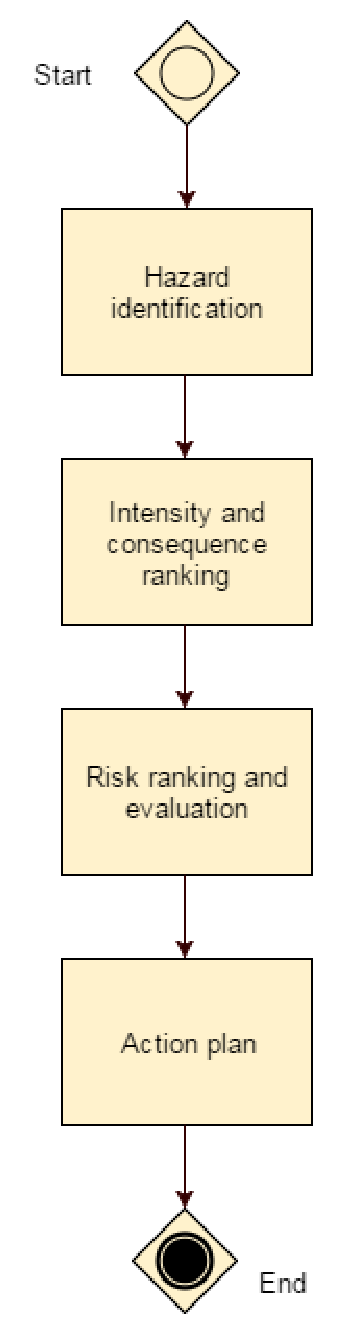
\includegraphics[scale=0.5]{risk-methodology} \caption{overarching risk methodology}
	\label{riskmethodology} 
\end{figure}

As can be seen from Figure \ref{riskmethodology}, the risk management plan involves four main work packages: 1) Hazard identification; 2) Intensity and consequence ranking; 3) Risk ranking and evaluation; and 4) Action plan. These work packages are supported with the steps described herein.

The step by step procedure for registering and evaluating hazard events and associated risks is itemized as follows

\begin{itemize}
	\item \underline{Step 1}: Register the hazard event into a designated field of the risk register table. Describe it as clear as possible and try to eliminate any ambiguity description of hazard;
	\item \underline{Step 2}: Register in words the consequences such hazards can bring into the project. This is important step as the description of consequence will provide stakeholders an insightful understanding on the impacts that hazards can cause;
	\item \underline{Step 3}: Define the levels of intensity and consequences for registered hazard events. These levels are considered when the hazard events have not been mitigated; 
	\item \underline{Step 4}: Register the current measurement (if any) against hazard events;
	\item \underline{Step 5}: Define the levels of intensity and consequences for registered hazard events in the case of having the measurement; 
	\item \underline{Step 6}: Frequently monitor the hazard events and their associated intensity and consequence to verify whether or not the levels reflecting the reality;
	\item \underline{Step 7}: Register the mitigation action/plan to minimize or eliminate hazard events. Mitigation action must be described in clear wording and must reflect what actually implementing on the construction site or in the office;
	\item \underline{Step 8}: Define the levels of intensity and consequences for registered hazard events in the case of having the mitigation action implemented.
\end{itemize}

The work packages and steps above should be placed in a continuous process for total quality management. It has a direct link to the Deming cycle (Plan-do-Check-Act) \citep{Walton1986}, and it is advisable for all stakeholders of the project to implement the cycle. An illustration of a Deming cycle for risk management is shown in Figure \ref{demingcyclerisk}.

\begin{figure}[!ht]
	\centering 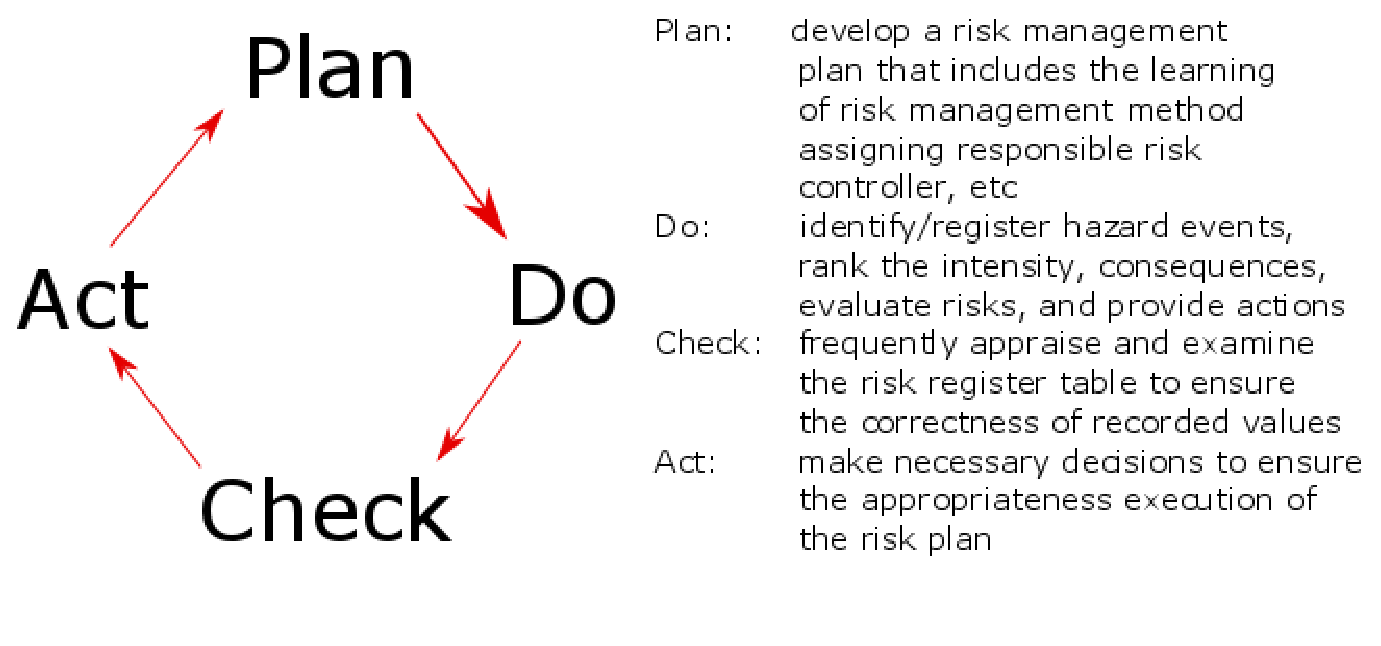
\includegraphics[scale=0.4]{demingcyclerisk} \caption{Deming cycle for risk management}
	\label{demingcyclerisk} 
\end{figure}

A risk management tool has been developed to allow project's stakeholders to actualize the risk management practices for any project. The tool was developed in Microsoft Excel environment, with embedded Visual Basic codes. Users can download the tool from the author's Github site \footnote{\linkurl{https://github.com/namkyodai}}. The details of the tool are presented along with the example in Section \ref{sec5}.

\section{Example}
\label{sec5}
\subsection{Project overview}
The project is to design and built a large scale water utilitiy project in a highly dense populated metropolitan city. There are three (3) major stakeholders involved in the project: 1) A Water Services company is the owner and operator of the plant; 2) the D\&B Contractor, who is an international consortium formed of a world reputable water engineering corporation and a local partner; 3) an EPCM (Engineering, Procurement, and Construction Management) Consultant to administer and supervise the work being executed by the D\&B Contractor. Other stakeholders include government regulators and private and public entities and local people living in the vicinity of the project. The project has been scheduled to complete in three (3) years, including design, construction, installation, and overall process proving phases.

As part of the requirements of the Owner, the Consultant is the one to facilitate the risk management task. However, to be clear, successful risk management is the responsibility of all stakeholders. Each stakeholder is responsible to take care of the four main tasks in risk management i.e. 1) Risk identification; 2) Risk ranking (including the evaluation on the likelihood and consequences); 3) Risk Evaluation; and 4) Risk mitigation.
\subsection{Intensity, Consequences, and Risk definitions}
\subsubsection{Intensity} \label{lik}
The intensity of an hazard event is defined in a range of 5, with 1 is the lowest level of intensity (very unlikely to occur) and 5 is the highest level of intensity (almost certain to occur). As mentioned in section \ref{sec3}, the intensity is a qualitative level of measuring how likely the hazard event can occur. It links directly to the likelihood (or probability). However, as probability value is hard to be quantified. It is practical to use a discrete scale to represent the quantitative nature of the probability. The range of 5 is good enough to represent the nature of likelihood as it is easy for managers and practical engineers to capture the sense of likelihood. The definition of the intensity is given in Table \ref{tbl_intensity}.

\begin{table}
	\centering
	\caption{Definition of intensity levels} 
	\begin{tabular}{l|p{2cm}|p{10cm}}
		\hline
		\multicolumn{1}{c|}{Scale} & \multicolumn{1}{c|}{Intensity level} & Definition \\ 
		\hline
		\multicolumn{1}{c|}{1} & \multicolumn{1}{c|}{Very unlikely} & Very unlikely, it can be assumed that it may not be experienced \\ 
		\multicolumn{1}{c|}{2} & \multicolumn{1}{c|}{Unlikely} & Unlikely to occur, stakeholders might have no experience of occurrence \\ 
		\multicolumn{1}{c|}{3} & \multicolumn{1}{c|}{Possible} & Possibly may occur, stakeholders have experience or knowledge of similar occurrence on other projects \\ 
		\multicolumn{1}{c|}{4} & \multicolumn{1}{c|}{Likely} & Likely to occur, stakeholders deem event likely to occur based on project specific circumstances \\ 
		\multicolumn{1}{c|}{5} & \multicolumn{1}{c|}{Almost certain} & Almost certain to occur \\ 
		\hline
	\end{tabular}
	\label{tbl_intensity}
\end{table}

\subsubsection{Consequences} \label{cons}
The consequence of an hazard event is also defined in a range of 5, with 1 is the lowest level of consequence (minor) and 5 is the highest level of consequence (catastrophic). As mentioned in section \ref{sec2}, the consequence is a qualitative level of measuring how the magnitude of loss incurred if a hazard event occur. Loss can be understood either as non-monetary units or monetary unit. In many practical cases, it is not straightforward to explicitly define an absolute value of monetary units for a level of consequence. In this regard, a better approach is to describe the consequence in an understandable definition for managers and engineers to capture the sense of how consequence will be after an occurrence of a hazard event. The definition of consequence used for the project is detailed in Table \ref{tbl_consequences}.

\begin{table}
	\centering
	\caption{Definition of consequence levels}
	\begin{tabular}{l|p{2cm}|p{10cm}}
		\hline
		\multicolumn{1}{c|}{Scale} & \multicolumn{1}{c|}{Consequence level} & Definition \\ 
		\hline
		\multicolumn{1}{c|}{1} & \multicolumn{1}{c|}{Minor} & Could result in injury or illness and not resulting in a lost work day. Small variation, delay of 1 day or less \\ 
		\multicolumn{1}{c|}{2} & \multicolumn{1}{c|}{Major} & Could result in injury or illness resulting in one or more lost work days, financial loss to 2 million Peso, delays up to 2 weeks \\ 
		\multicolumn{1}{c|}{3} & \multicolumn{1}{c|}{Severe} & Could result in permanent disability, major financial loss, severe project consequences to time (delays greater than 2 weeks up to 2 months) losses up to 5 million Peso \\ 
		\multicolumn{1}{c|}{4} & \multicolumn{1}{c|}{Critical} & Could result in disability, great financial and reputational loss, serious project consequences to budget and time exceeding 2 months \\ 
		\multicolumn{1}{c|}{5} & \multicolumn{1}{c|}{Catastrophic} & Could result in fatality, irrecoverable financial and reputational loss, project shutdown for in-determinant duration \\ 
		\hline
	\end{tabular}
	\label{tbl_consequences}
\end{table}
\subsubsection{Risk matrices}
By definition, risk is the multiplication of probability and consequences. This infers that both probability and consequences must be measurable. In addition, the probability must take a space between 0 and 1 and the consequences must be measurable in term of lost in monetary units. However, as earlier mentioned in section \ref{sec3} and subsections \ref{lik} and \ref{cons},  risks being considered in any construction project are not direct multiplications of the scale of the likelihood and consequence. For practical use, instead of multiplying the likelihood and consequence to derive the risk, it is persuasive and practical to use combination of intensity and consequence to define risk. The definition of risks as a set of combinations of the scale of the intensity and the scale of consequence is given in Table \ref{tbl_risks}.

\begin{table}
	\centering
	\caption{Definition of risk levels (risk matrices)}
	\begin{tabular}{l|l|l|l|l|l|l}
		\hline
		Intensity &  & \multicolumn{5}{c}{Consequences} \\ 
		\cline{3-7}
		&  & Minor & Major & Severe & Critical & Catastrophic \\ 
		\cline{3-7}
		& \multicolumn{1}{c|}{Scale} & \multicolumn{1}{c|}{1} & \multicolumn{1}{c|}{2} & \multicolumn{1}{c|}{3} & \multicolumn{1}{c|}{4} & \multicolumn{1}{c}{5} \\ 
		\hline
		Almost Certain & \multicolumn{1}{c|}{5} & \multicolumn{1}{c|}{\cellcolor{brown}\color{white}8} & \multicolumn{1}{c|}{\cellcolor{blue}\color{white}16} & \multicolumn{1}{c|}{\cellcolor{violet}\color{white}20} & \multicolumn{1}{c|}{\cellcolor{black}\color{white}22} & \multicolumn{1}{c}{\cellcolor{black}\color{white}25} \\ 
		\hline
		Likely & \multicolumn{1}{c|}{4} & \multicolumn{1}{c|}{\cellcolor{brown}\color{white}7} & \multicolumn{1}{c|}{\cellcolor{brown}\color{white}9} & \multicolumn{1}{c|}{\cellcolor{violet}\color{white}18} & \multicolumn{1}{c|}{\cellcolor{violet}\color{white}21} & \multicolumn{1}{c}{\cellcolor{black}\color{white}24} \\ 
		\hline
		Possible & \multicolumn{1}{c|}{3} & \multicolumn{1}{c|}{\cellcolor{green}\color{black}4} & \multicolumn{1}{c|}{\cellcolor{brown}\color{white}6} & \multicolumn{1}{c|}{\cellcolor{blue}\color{white}12} & \multicolumn{1}{c|}{\cellcolor{violet}\color{white}17} & \multicolumn{1}{c}{\cellcolor{black}\color{white}23} \\ 
		\hline
		Unlikely & \multicolumn{1}{c|}{2} & \multicolumn{1}{c|}{\cellcolor{green}\color{black}2} & \multicolumn{1}{c|}{\cellcolor{green}\color{black}5} & \multicolumn{1}{c|}{\cellcolor{brown}\color{white}11} & \multicolumn{1}{c|}{\cellcolor{blue}\color{white}15} & \multicolumn{1}{c}{\cellcolor{violet}\color{white}19} \\ 
		\hline
		Very unlikely & \multicolumn{1}{c|}{1} & \multicolumn{1}{c|}{\cellcolor{green}\color{black}1} & \multicolumn{1}{c|}{\cellcolor{green}\color{black}3} & \multicolumn{1}{c|}{\cellcolor{brown}\color{white}10} & \multicolumn{1}{c|}{\cellcolor{blue}\color{white}13} & \multicolumn{1}{c}{\cellcolor{blue}\color{white}14} \\ 
		\hline
	\end{tabular}
	\label{tbl_risks}
\end{table}
For the purpose of visualization, each level of risk is coded with a distinct color, which is also depicted in the table. These ranges of colors associated with risks will be used to pain the background of cells. Users can define their own choices of colors by directly change the background colors in the risk matrices of worksheet "\underline{definition}" of the risk tool. This range of colors will later be used to provide eye-catching visualization of risks in the "\underline{risk register worksheet}" and "\underline{risk profile worksheet}", which will be shown in sub-sequence subsections.

\subsection{Risk Register and Risk Reduction Management Framework} \label{subriskregister}
\subsubsection{Risk Register}
As the project progresses daily, weekly, and monthly, the levels of intensity associated with hazard events will change and also the levels of consequence. The changes in the level of intensity and consequence for each risk can happen based on the nature of the works, the current measurement against such hazard events, and the actual implementation of risk mitigation action. Such changes must be recorded and evaluated in "\underline{risk register}" worksheet. 

The risk register worksheet is the work space that users can enter/register new hazard event per row. Upon registering new hazard event, users can define its the current measurement against such event as well as the mitigation action to mitigate or minimize the exposure of risk. In a nutshell, there are 3 distinct fields (unmitigated, current, and mitigated) for each hazard event. Along with these fields are levels of intensities and consequences. 

As the matter of fact, the level of intensity and consequence must be in descending order. For the sake of demonstration, a typical hazard event is given herewith. For example, during the construction phase, it is always likely that a major accident can occur, this is a safety issue and such a hazard should be registered with a highest level of intensity (5 is the highest level in intensity scale). Impacts or consequences incurred as a result of the accident could be a fatality loss, which in turn imposes a serious impact to stakeholders and might cause  significant delay of the project, as such the level of consequence is 5. The combination of 5x5, per the definition Table \ref{tbl_risks}, is 25. 

Next the users check if there exists a set of measurement against such a safety issue. Measurement against safety issue is normally written in the form of safety and occupational health guideline. This guideline is, in most of the case, imposed to all stakeholders and they have to read/learn it before entering the construction site for executing the works. This means, thanks to having the measurement, it is expected that both the intensity and consequences can be reduced to a certain level (e.g. levels of intensity and consequence are 4 and 5, respectively). The last step in this process is to implement the practical action against the hazard (e.g. assign safety controllers to different areas of work, strictly impose the safety and occupational health plan, weekly or monthly organizing short on-site safety meeting). 

Aside from the steps described in earlier section, users can have their flexibility to register each hazard under a set of categories and assign risks to be under specified stakeholders for convenience of monitoring and control. An example of how to organize such a set of categories is shown in the Table \ref{tbl_categories}
\begin{table}
	\centering
	\caption{Grouping and classifying hazard events}
	\begin{tabular}{l|l|l}
		\hline
		Risk categories & \multicolumn{1}{c|}{Team} & Chair person \\ 
		\hline
		Approvals & \multicolumn{1}{c|}{A} &  \\ 
		Planning, scoping & \multicolumn{1}{c|}{A} &  \\ 
		Stakeholders & \multicolumn{1}{c|}{A} &  \\ 
		Commissioning & \multicolumn{1}{c|}{B} &  \\ 
		Detailed design & \multicolumn{1}{c|}{B} &  \\ 
		Construction & \multicolumn{1}{c|}{C} &  \\ 
		Procurement & \multicolumn{1}{c|}{C} &  \\ 
		Delivery & \multicolumn{1}{c|}{D} &  \\ 
		Environment & \multicolumn{1}{c|}{D} &  \\ 
		\hline
	\end{tabular}
	\label{tbl_categories}
\end{table}

Having such a set of categories will also provide convenience for project managers and project directors to organize regular interim risk workshops and give a clear message of risks to each and every team, who must be responsible for implementing an effective risk management plan.

An extracted part of the risk register worksheet for the project is shown in Figure \ref{fig_riskregister}.


\begin{sidewaysfigure}[!ht]
	\centering 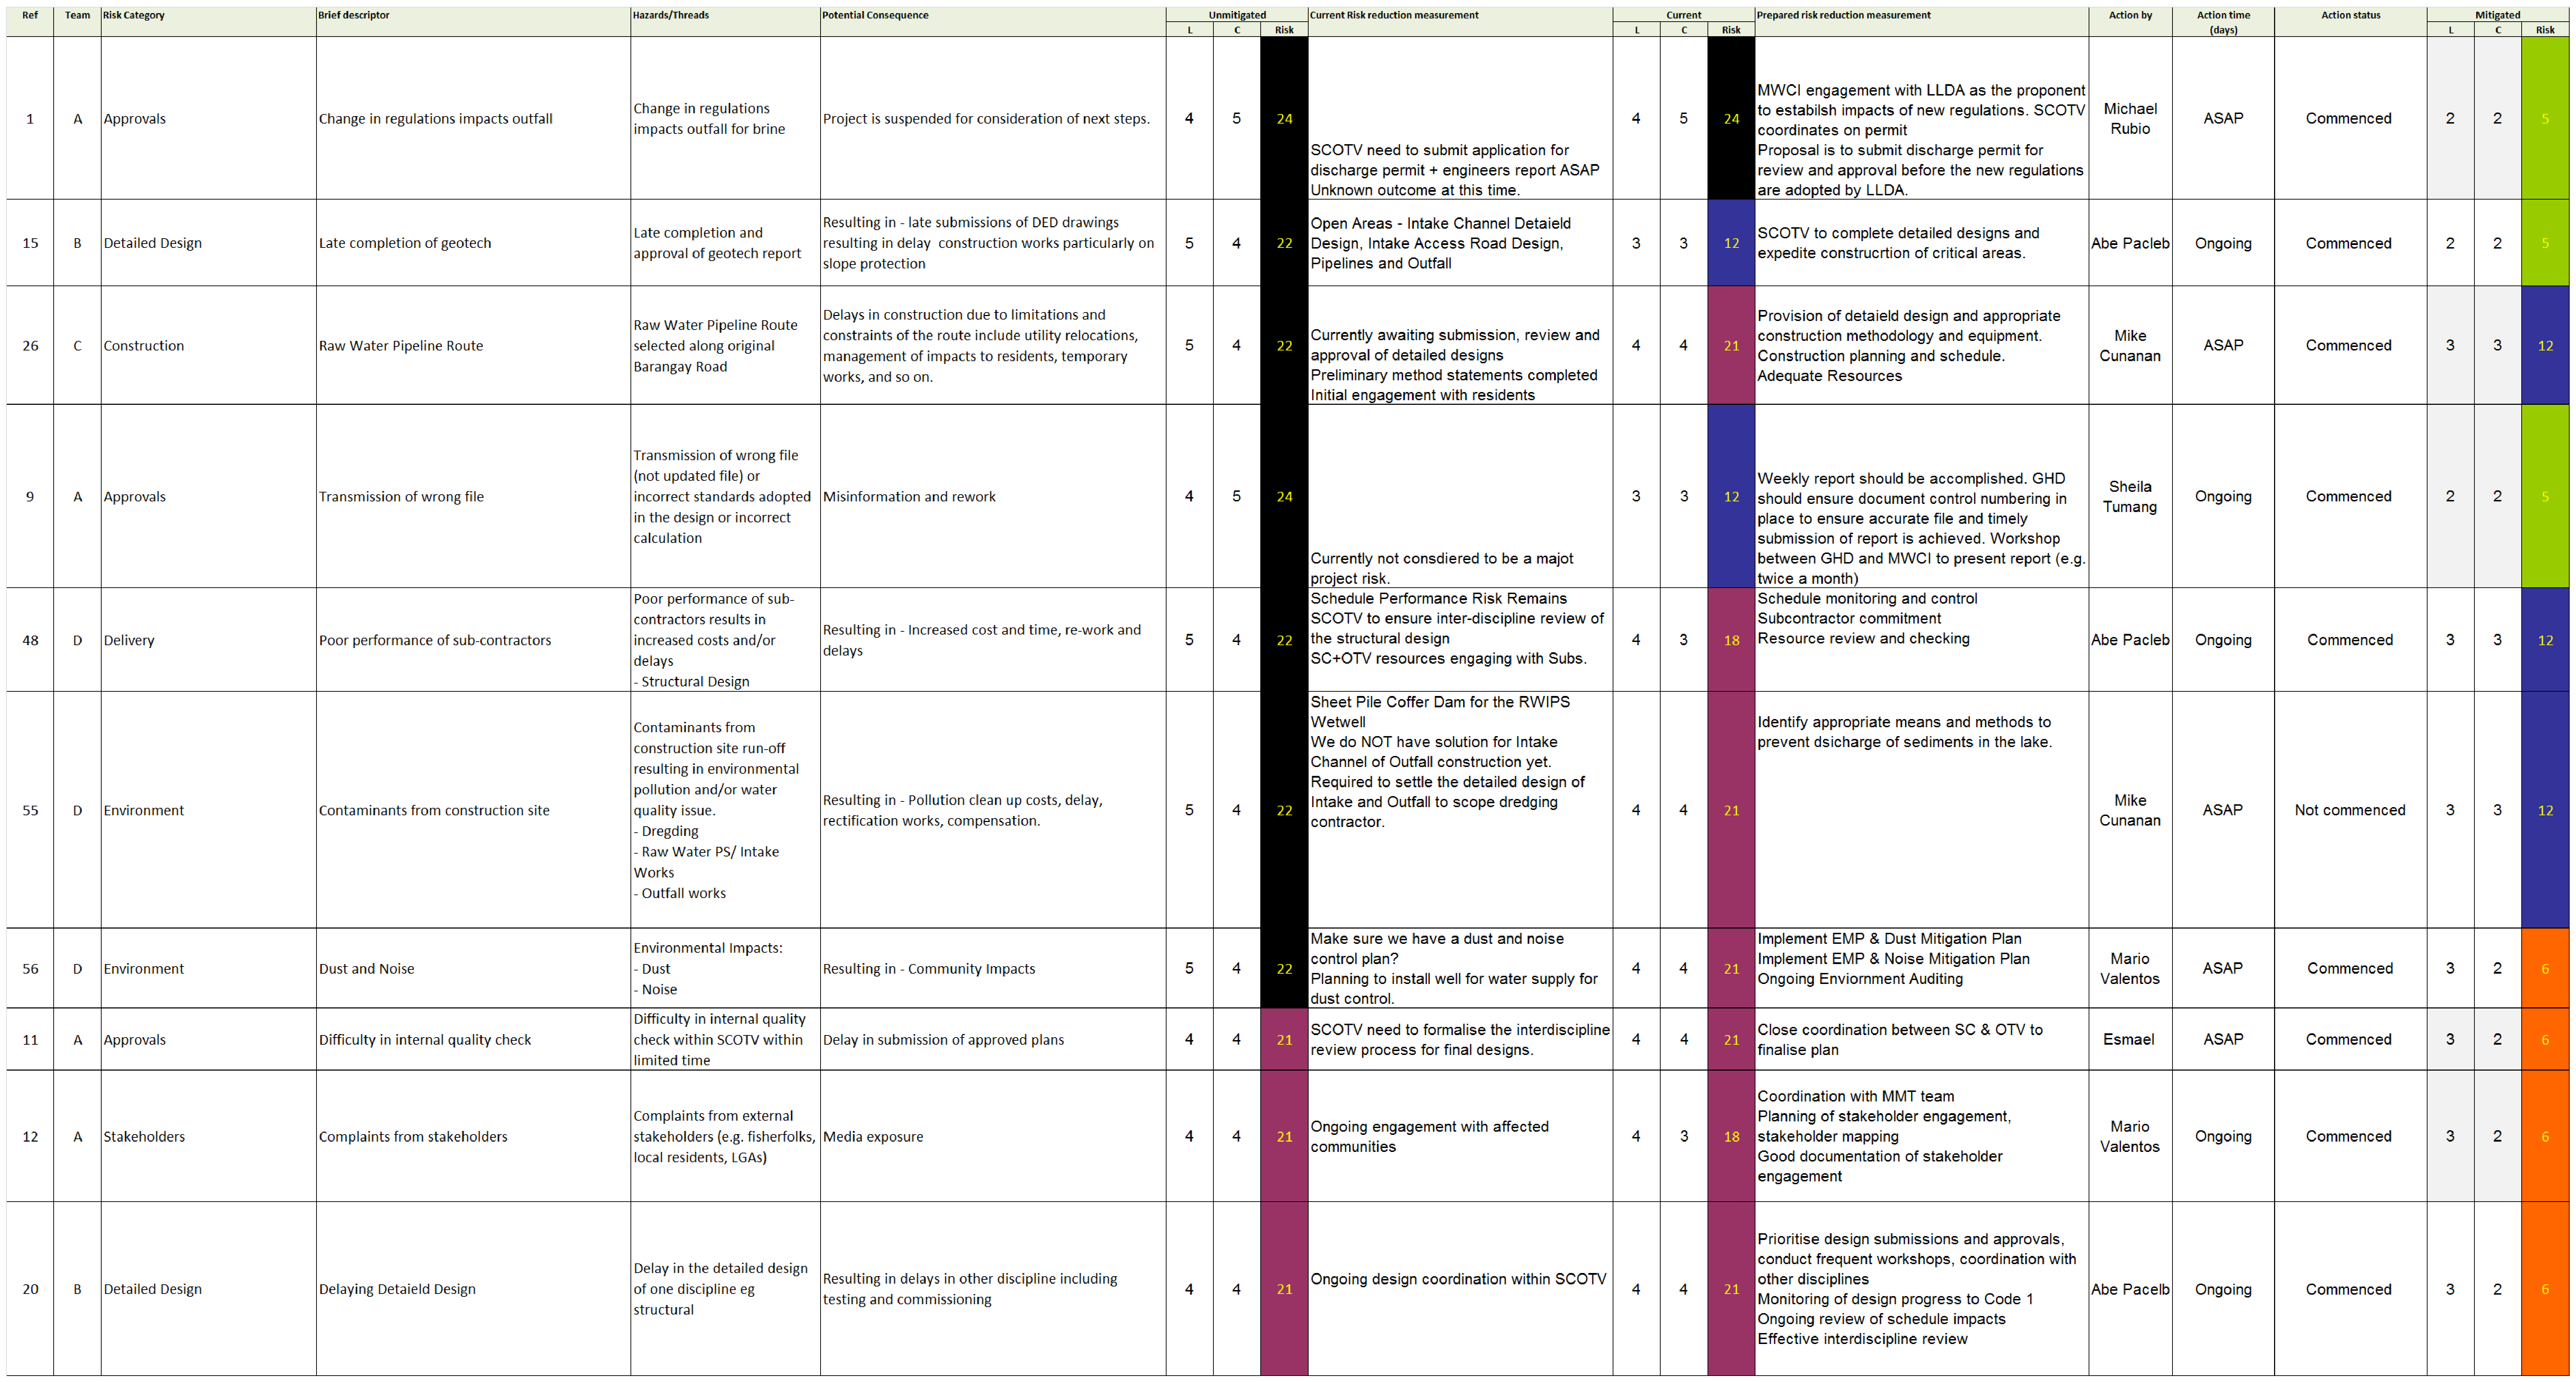
\includegraphics[scale=0.2]{riskregister} \caption{Part of risk register worksheet}
	\label{fig_riskregister} 
\end{sidewaysfigure}

\subsubsection{Risk Reduction Management Framework}
The process involved with using the Risk Register as described above can be summarized in a framework with its order as follows
\begin{itemize}
	\item Risk register: register new risk events into the worksheet;
	\item Risk reduction: remove or change risk events and their associated reduction methodology/activities to reflect up-to-date status and condition (e.g. intensity and consequence);
	\item Risk mitigation: formulate mitigation strategies by means of planning, providing training, PPCs, etc;
	\item Risk management: manage the residual risk with proactive supervision, communication, and on-the-spot action.
	
\end{itemize}

\subsection{Risk Profile}
Risk profile is a worksheet summarizing the results of all previous steps described in subsection \ref{subriskregister}. Further than that, it has been designed to provide a graphical visualization of risks, which serves as a good way to describe the importance of each and every risk incurred in any phase of a project. The graphical representation of risk provides an ease for project managers and directors to summary the risks and action plans in a report form, which is often required by the Owners.

An extracted part of the risk profile worksheet for the project is shown in Figure \ref{fig_riskprofile}.

\begin{sidewaysfigure}[!ht]
	\centering 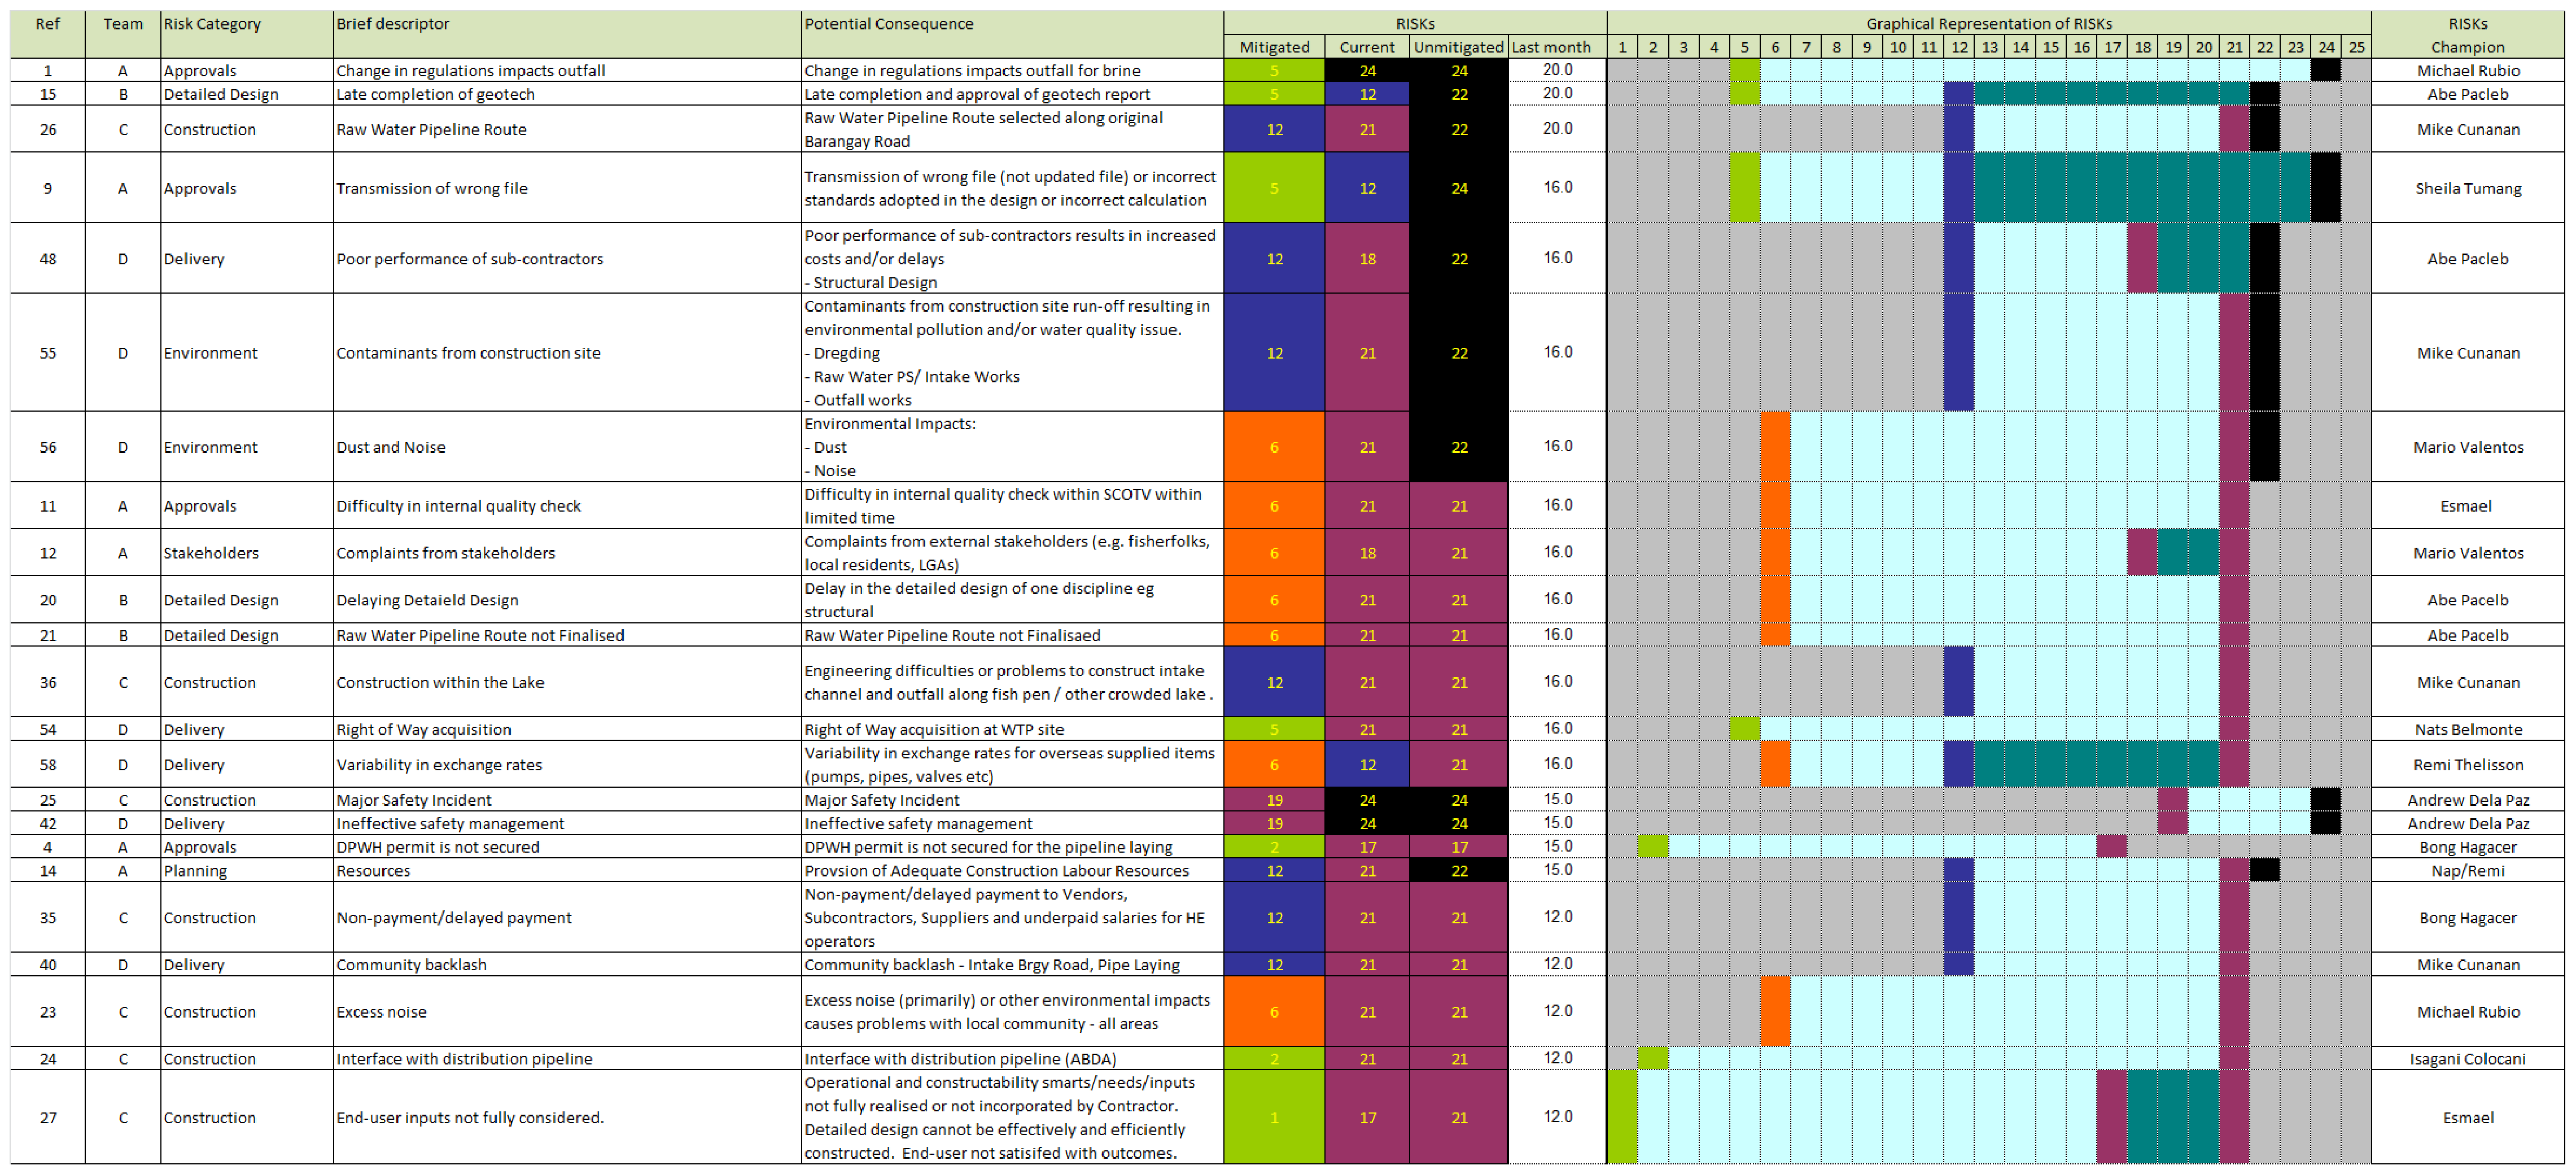
\includegraphics[scale=0.3]{riskprofile} \caption{Part of risk profile worksheet}
	\label{fig_riskprofile} 
\end{sidewaysfigure}

\section{Conclusion}
\label{sec6}
This paper presents a risk management methodology and a risk tool that can be used for risk control and management of large scale construction projects. The methodology was developed aiming for practical application. The methodology is different from the conventional methodology in the way of defining risks as combination of intensity and consequence but not on the multiplication of likelihood and consequence, which has been proved to be incorrect. A risk tool was developed using Excel VBA and is released as an open source code for the community. It has a friendly user-interface to help project managers and directors as well as engineers to implement risk management plans in practical situation. The methodology and the tool has been successfully implemented for a large scale construction project in a mega urban city.  


%\section*{Acknowledgment}
%This work was funded by Manila office of GHD Ply ltd. The authors would like to thank the Country Manager (Mr. Carl Willis) and members of Mining and Civil Group and Water Resources Group for their generous supports during the course of developing this work.
%\label{sec7}

\section{Data Availability Statements}
Data generated by the authors or analyzed during the study are available at the author's github respository:  (https://github.com/namkyodai/PracticalRISK)


\bibliographystyle{plainnat} % or try abbrvnat or unsrtnat
\bibliography{ghdreference} % refers to example.bib

\end{document}